\section{Griffin inverse-transformation wall function}
\label{sec:wall-functions:griffin}

Griffin et al. construct a compressible near-wall profile by applying an inverse velocity transformation to an incompressible wall law and closing the temperature profile through an algebraic temperature--velocity relation~\cite{griffin2022WFbrief,griffin2023WF}. The formulation accounts for density and viscosity variations associated with wall cooling while retaining a unified description of the viscous sublayer, buffer layer and logarithmic region. Its application here as a RANS wall function requires both the local matching state and information about the boundary layer edge.

\subsection{Momentum and thermal closures}
\label{subsec:wall-functions:griffin:governing-relations}

The momentum closure builds on the total-stress velocity transformation of Griffin et al.~\cite[Eqs.~(4)--(5)]{griffin2021Transformation}. It combines viscous scaling near the wall with turbulence-equilibrium scaling in the logarithmic region, blending between them through the buffer layer. The wall model uses its approximately constant-total-shear-stress form. Inverting this transformation converts the mean shear of a damped incompressible eddy-viscosity model into the compressible velocity gradient, including local density and viscosity variations~\cite[Eq.~(2.2)]{griffin2023WF}. The viscous limit recovers the linear wall law; the model is therefore not restricted by construction to logarithmic-layer sampling.
\par\medskip

The thermal closure is a quadratic temperature--velocity relation based on the generalized Reynolds analogy~\cite[Eq.~(2.5)]{griffin2023WF}. It satisfies the wall temperature and the sampled temperature at the matching velocity, while its wall slope is prescribed through the Reynolds analogy factor and the recovery temperature. The latter depends on the edge velocity and temperature. This wall slope links heat-flux directly to wall shear, without solving a separate temperature equation with an assumed constant turbulent Prandtl number. In Griffin's convention, heat-flux is positive into the fluid and negative for a cooled wall.
\par\medskip

For a prescribed wall temperature, the inputs are the velocity, temperature and density at the physical matching height \(y_m\), the edge state, an equation of state and a viscosity law. The inner reconstruction uses the ideal-gas law with approximately constant pressure and constant specific heat. A trial wall shear stress is used to integrate the inverse relation from the wall region to \(y_m\), updating temperature and transport properties along the reconstructed profile. The stress is iterated until the integrated velocity reproduces the sampled velocity; the thermal relation then supplies the heat-flux~\cite[Section~2.3]{griffin2023WF}. Both wall loads thus follow from reconstructed wall slopes rather than a wall-to-cell secant.
\par\medskip

The implementation retains the Reynolds-number-dependent calibration of the incompressible coefficients \(\kappa\) and \(A^+\) from the earlier research brief~\cite[Section~2]{griffin2022WFbrief}. These coefficients are selected using the edge-based semi-local friction Reynolds number, so the estimated thickness also enters the closure. The journal article examines this calibration but adopts fixed values \(\kappa=0.41\) and \(A^+=17\) for its subsequent simulations~\cite[Section~3]{griffin2023WF}. This distinction matters when comparing the implemented variant with published results.

\subsection{Boundary layer edge reconstruction and sensitivity}
\label{subsec:wall-functions:griffin:edge-detection}
\label{para:Griffin-BL-edge}

The edge quantities are obtained with Griffin et al.'s local-reconstruction method~\cite{griffin2021BLthickness}. It reconstructs a local inviscid velocity \(U_I\) from the stagnation enthalpy and identifies \(\delta_{99}\) where the actual tangential velocity first satisfies \(U/U_I=0.99\)~\cite[Eq.~(9) and Appendix~D, Eqs.~(D1)--(D2)]{griffin2021BLthickness}. This replaces comparison with a prescribed freestream velocity and permits a varying inviscid outer profile. The compressible construction assumes an inviscid, non-heat-conducting outer flow.
\par\medskip

In the present finite-volume implementation, cell-centre states are sampled outward from the wall, and their maximum stagnation enthalpy supplies the reconstruction reference. The first crossing of the squared velocity-ratio criterion brackets the edge. Its position, velocity and temperature are obtained by linear interpolation between the bracketing samples, using the squared ratio as interpolation coordinate. This interpolation is an implementation choice; the continuous edge criterion does not prescribe a discrete interpolation scheme.
\par\medskip

Figure~\ref{fig:wfs:BL_edge_quantities} illustrates the sensitivity for M6Tw025. The extracted thickness and edge temperature vary appreciably between conventional wall-function meshes, whereas the relative variation in edge velocity is smaller. These differences reflect both changes in the computed profiles and their discrete reconstruction; they do not isolate interpolation error. The two DNS markers further show that edge quantities must be compared using consistent definitions.
\par\medskip

These variations affect model inputs: edge velocity and temperature enter the thermal closure through the recovery temperature, and thickness enters the coefficient calibration described above. The physical matching height remains a separate input. The figure identifies an additional mesh dependence, but does not establish which edge quantity dominates the wall-flux error. This motivates separating the prescribed-profile closure tests in Section~\ref{sec:comparative:zpg:cross-comparison} from the coupled mesh assessment in Section~\ref{subsec:comparative:zpg:yplus-sensitivity}.

\begin{figure}[H]
    \centering
    % Figure provenance (WSL; absolute paths):
    %   Original export: /home/mgnadlinger/Xue_et_al/flat_plate/M6Tw025/validation/outputs_Griffin_SA/reported_edge_quantities.png
    %   Retained generator: /home/mgnadlinger/WF_validation/LowH_M3/Griffin_SA/analyze_griffin_edge_diagnostics.py
    %   Generator's original data root: /home/michael_gnadlinger/Xue_et_al/flat_plate/M6Tw025/WF/Griffin_SA
    %   Generator's original wall-resolved root: /home/michael_gnadlinger/TM_verification/SA/Zhang/M6Tw025_mesh_sens/5e-4_dx5
    %   Note: Retained export and generator checked; the exact companion CSV was not located.
    %   Note: The plotted DNS station is x=0.206771 m, distinct from the later matched comparison station.
    % End figure provenance.
    % Caption-sized typography (2026-10-19): 10 pt at 170 mm manuscript width.
    % Retained high-resolution curve pixels with vector labels and legend;
    % local source and audit: 05_WF_Idea_Implementation/griffin_edge_sources/.
    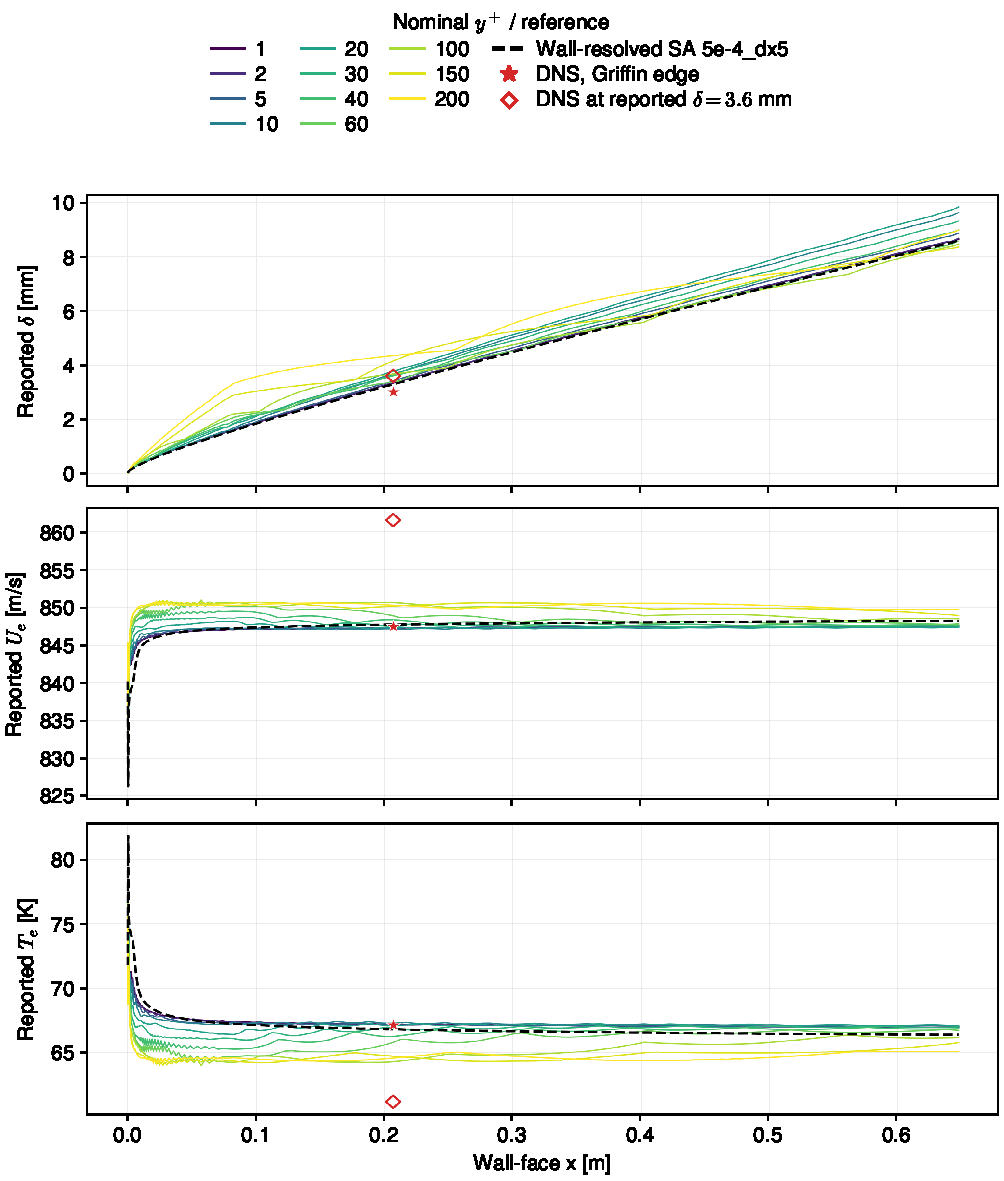
\includegraphics[width=\linewidth]{05_WF_Idea_Implementation/Griffin_Wallfunction_Edge_Quantities.pdf}
    \caption[Mesh sensitivity of the Griffin edge quantities]{Boundary layer thickness \(\delta\), edge velocity \(U_e\) and edge temperature \(T_e\) for M6Tw025. Colours identify conventional meshes by nominal first-cell \(y_1^+\); the dashed curve is the wall-resolved SA reference evaluated with the same criterion. Stars apply the Griffin criterion to the DNS profile, taking the unavailable mean wall-normal velocity as zero. Diamonds show the reported DNS thickness \(\delta=3.6\,\mathrm{mm}\) and the velocity and temperature interpolated at that height~\cite{zhang2018direct}.}
    \label{fig:wfs:BL_edge_quantities}
\end{figure}

\subsection{Application to RANS and limits of the published validation}
\label{subsec:wall-functions:griffin:validation-scope}

Griffin et al. describe the model as suitable for coupling to either LES or RANS. Their assessment combines a-priori tests on prescribed DNS profiles with a-posteriori WMLES of turbulent channels; it contains no coupled RANS validation~\cite[Sections~3--5]{griffin2023WF}. The principal comparisons use \(y_m=0.3\delta\), but the journal article also varies matching height during mesh refinement, including \(0.15\delta\) and \(0.075\delta\)~\cite[Section~4.1]{griffin2023WF}. These are matching locations, not prescribed first-cell-centre heights. As in WMLES it is common practice to retain off-wall resolutions below the point at which the wall model samples the boundary layer and then select the sample station adaptively dependant on the local boundary layer behaviour, i.e. if detachment is detected \cite{gao2026adaptive}. In addition to LES commonly using higher-order reconstruction methods, this may explain why Griffin et al. most likely didn't stumble upon  same mesh requirement issue (ref. Section \ref{subsec:comparative:zpg:yplus-sensitivity}).
\par\medskip

Here, the closure is coupled to SA through the near-wall turbulence constraint, with its wall shear and heat-flux delivered directly to HiSA as described in Section~\ref{subsec:wall-functions:direct-flux-delivery}. This RANS coupling and the reconstructed edge inputs require their own assessment. The published WMLES performance consequently provides no direct validation of the complete implementation. Nevertheless, the standalone closure can be checked against the published a-priori results, as shown in Table~\ref{tab:erriso:Griffin-a-priori-validation}. That consistency check supports the subsequent error-isolation study without implying equivalent accuracy of the coupled RANS calculations.
